\title{Machine Learning Spring 2019 HW1}
\author{
        Yueh Cheng Liu \\
        National Taiwain University\\
}
\date{\today}
\documentclass[12pt]{article}
\usepackage{amsmath}
\usepackage{bbm}
\usepackage{graphicx}
\usepackage{bm}
\begin{document}
\maketitle

% \begin{abstract}
% This is the paper's abstraasdsadsct \ldots
% \end{abstract}

\section*{1}
\begin{center}
    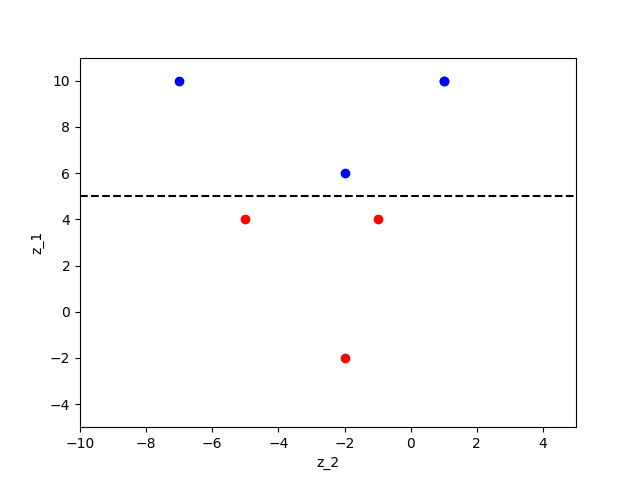
\includegraphics[scale=0.5]{p1.png} 
\end{center}
The equation of the hyperplane is $z_1=5$. Which has the largest margin $2$.
If the hyperplane slightly rotate clockwisely or counter-clockwisely, the margin will be shrinking due to the two red points $(4, -4)$ and $(4, -1)$.

\section*{2}
$\bm{\alpha} = (0, 0.704, 0.704, 0.889, 0.259, 0.259, 0)$. $x_i$ with $i=2,...,6$ are the support vectors. 

\section*{3}
\begin{equation*}
\begin{split}
    \sum_{n\in \textbf{SV}} \alpha_n y_n K(x_n, \bm{x})+b 
    &= \sum_{n\in \textbf{SV}} \alpha_n y_n (1+x_n^T \bm{x})^2+b \\
    &= \sum_{n\in \textbf{SV}} \alpha_n y_n (1 +x_n^T \bm{x} + (x_n^T \bm{x})(x_n^T \bm{x}))+b
\end{split}
\end{equation*}
Let $\bm{x} = (x_1, x_2)$ and replace the $\alpha_n$, $y_n$, $x_n$ with number.

\begin{equation*}
\begin{split}
    \sum_{n\in \textbf{SV}} \alpha_n y_n (1 +x_n^T \bm{x} + (x_n^T \bm{x})(x_n^T \bm{x}))
    &= -0.704 \cdot ( 1 + x_2 + x_2^2) \\
    &-0.704 \cdot (1 + -x_2 + x_2^2) \\ 
    &+ 0.889 \cdot (1 + -x_1 + x_1^2) \\ 
    &+ 0.259 \cdot (1 + 2x_2 + 4x_2^2) \\ 
    &+ 0.259 \cdot (1 + -2x_2 + 4x_2^2) \\ 
    &= -1 - 0.889 x_1 + 0.889 x_1^2 + 0.664 x_2^2
\end{split}
\end{equation*}

and take a support vector $x_2 = (0, 1)$ to calculate $b$.

\begin{equation*}
\begin{split}
   b &= y_s - \sum_{n=1}^{N} \alpha_n y_n K(x_n, x_s) \\
   &= y_s - \sum_{n=1}^{N} \alpha_n y_n (1 +x_n^T x_s + (x_n^T x_s)(x_n^T x_s)) \\
   &= -1 - \sum_{n=1}^{N} \alpha_n y_n (1 +x_{n,2} + x_{n,2}^2) \\
   &= 0.663
\end{split}
\end{equation*}
So the curve is $0.889 x_1 + 0.889 x_1^2 + 0.664 x_2^2 - 0.337 = 0$.

\section*{4}
The curve found in (1) is $2x_2^2 - 4x_1 - 3 = 0$. Which is not the same with (2).
The transformation (2) represented by the kernel function is different from the transformation in (1),
so the optimal separating hyperplanes for them are different.
\section*{5}
\begin{equation*}
\begin{split}
|| \tilde{\phi}(x) ||^2 &= 1 + \frac{2}{1!} x^2 + \frac{2^2}{2!} x^4 + ... \\
&= \sum_{n=0}^\infty \frac{2^n}{n!} x^{2n}
\end{split}
\end{equation*}

Let $y=x^2$ and subsitude $x$ with $y$. 

\begin{equation*}
\begin{split}
\sum_{n=0}^\infty \frac{2^n}{n!} x^{2n} &= \sum_{n=0}^\infty \frac{2^n}{n!} y^{n} \\
&= e^{2y} \\
&= e^{2x^2}
\end{split}
\end{equation*}

So that 
\[  e^{x^2} = || \tilde{\phi}(x) ||\]

\section*{6}
\[ cos(x', x) = \frac{{x'}^Tx}{|x'||x|}\]
The transform function $\phi(x)$ is $\frac{x}{|x|}$. 

\section*{7}
\[ L(R, c, \lambda) = R^2 + \sum_{n=1}^N \lambda_n (||z_n - c||^2 - R^2) \]

\section*{8}
\begin{itemize}
\item Primal feasible: $||z_n - c||^2 \leq R^2$ 
\item Dual feasible: $\lambda_n \geq 0$ for $n = 1, 2, ..., N$
\item Dual-inner optimal: 
\[ \frac{\delta L(R, c, \lambda)}{\delta c} = 0 = \sum_{n=1}^N \lambda_n (-2z_n + 2c) \]
\begin{equation} \label{eq:1}
c \sum_{n=1}^N \lambda_n = \sum_{n=1}^N \lambda_n z_n 
\end{equation}
\[ \frac{\delta L(R, c, \lambda)}{\delta R} = 0 = 2R - \sum_{n=1}^N \lambda_n 2R \]
\begin{equation} \label{eq:2}
R(1 - \sum_{n=1}^N \lambda_n) = 0 
\end{equation}

By equation \ref{eq:1}, if $\sum_{n=1}^N \lambda_n \neq 0$, then $c = \frac{\sum_{n=1}^N \lambda_n z_n}{\sum_{n=1}^N \lambda_n}$

\item Primal-inner opitmal:
\[ \frac{\delta L(R, c, \lambda)}{\delta \lambda_n} = 0 = ||z_n - c||^2 - R^2  \]
\end{itemize}

\section*{9}
By equation \ref{eq:2}, if $R > 0$ then $\sum_{n=1}^N \lambda_n = 1$ and thus $c = \frac{\sum_{n=1}^N \lambda_n z_n}{\sum_{n=1}^N \lambda_n} = \sum_{n=1}^N \lambda_n z_n$.

\begin{equation*}
\begin{split}
L(R, c, \lambda) 
&= R^2 - R^2\sum_{n=1}^N \lambda_n + \sum_{n=1}^N \lambda_n (z_n^Tz_n - 2z_n^Tc + c^Tc) \\
&= \sum_{n=1}^N \lambda_n (z_n^Tz_n - 2z_n^Tc + c^Tc) \\
&= \sum_{n=1}^N \lambda_n (z_n^Tz_n - 2z_n^T \sum_{i=1}^N \lambda_i z_i + \sum_{i=1}^N \sum_{j=1}^N \lambda_i z_i^T  \lambda_j z_j) \\
&= \sum_{n=1}^N \lambda_n z_n^Tz_n - 2 \sum_{n=1}^N \lambda_n z_n^T \sum_{i=1}^N \lambda_i z_i + \sum_{i=1}^N \sum_{j=1}^N \lambda_i \lambda_j z_i^T z_j \\
&= \sum_{n=1}^N \lambda_n z_n^Tz_n - \sum_{i=1}^N \sum_{j=1}^N \lambda_i \lambda_j z_i^T z_j 
\end{split}
\end{equation*}

which $\sum_{n=1}^N \lambda_n = 1$.

\section*{10}

By the KKT condition of primal-inner optimal $0 = ||z_i - c||^2 - R^2$.
\begin{equation*}
\begin{split}
    R &= ||z_i - c|| \\
    &= (z_i^Tz_i - 2z_i^Tc + c^Tc)^{\frac{1}{2}} \\
    &= (z_i^Tz_i - 2z_i^T \sum_{n=1}^N \lambda_n z_n + \sum_{i=n}^N \sum_{m=1}^N \lambda_n \lambda_m z_n^T z_m)^{\frac{1}{2}} \\
    &= \Big(K(x_i, x_i) - 2 \sum_{n=1}^N \lambda_n K(x_i, x_n) + \sum_{n=1}^N \sum_{m=1}^N \lambda_n \lambda_m K(x_n, x_m)\Big)^{\frac{1}{2}} 
\end{split}
\end{equation*}

\section*{11}
The dual problem of hard-margin and soft-margin SVM are almost the same.
The only difference is soft-margin has one more contraint which is $\alpha_n \leq C$ for $n=1,...,N$.
Therefore, when the optimal $\alpha_n^*$ in the hard-margin SVM satisfy $C \geq max_{1\leq n \leq N} \alpha_n^*$ which will also satisfy $\alpha_n \leq C$ for $n=1,...,N$
and the $\alpha_n^*$ will also be the optimal solution of soft-margin SVM.

\section*{12}
The original minimization objective of soft-margin SVM is
\begin{equation} \label{eq:1}
    \frac{1}{2} \bm{\alpha}^T Q \bm{\alpha} - \mathbbm{1}^T \bm{\alpha}
\end{equation}
Let the new objective of soft-margin with new kernel $\tilde{K} (x, x') = pK(x, x')$ and new $\tilde{C} = \frac{C}{p}$ be
\begin{equation} \label{eq:2}
    \begin{split}
        \frac{1}{2} \bm{\alpha}'^T Q' \bm{\alpha}' - \mathbbm{1}^T \bm{\alpha}' 
        &= \frac{1}{2} \bm{\alpha}'^T pQ \bm{\alpha}' - \mathbbm{1}^T \bm{\alpha}' \\
        &= \frac{1}{p} \bigg( \frac{1}{2} (p\bm{\alpha}')^T Q (p\bm{\alpha}') - \mathbbm{1}^T (p\bm{\alpha}') \bigg)
    \end{split}
\end{equation}
Since $\frac{1}{p}$ constant in (\ref{eq:2}) can be ignored, the objective function of (\ref{eq:1}) is equivalent to (\ref{eq:2}) in the case of $\alpha' = \frac{\alpha}{p}$. And $\alpha'$ also satisfies the condition of $C'$.
\begin{equation*}
    0 \leq \alpha' = \frac{\alpha}{p} \leq C' = \frac{C}{p} 
\end{equation*}

The new decision function $f(x)$ is equivalent to the original decision function $f(x)$. 
\begin{equation*}
\begin{split}
    f'(x) &= \sum_{\text{SV indices n}} \alpha_n' y_n \tilde{K}(x_n, x) + y_s - \sum_{\text{SV indices n}} \alpha_n' y_n \tilde{K}(x_n, x_s) \\
    &= \sum_{\text{SV indices n}} \alpha_n y_n K(x_n, x) + y_s - \sum_{\text{SV indices n}} \alpha_n y_n K(x_n, x_s) \\
    &= f(x)
\end{split}
\end{equation*}
which $(x_s, y_s)$ is a free support vector.


\section*{13}
\begin{center}
    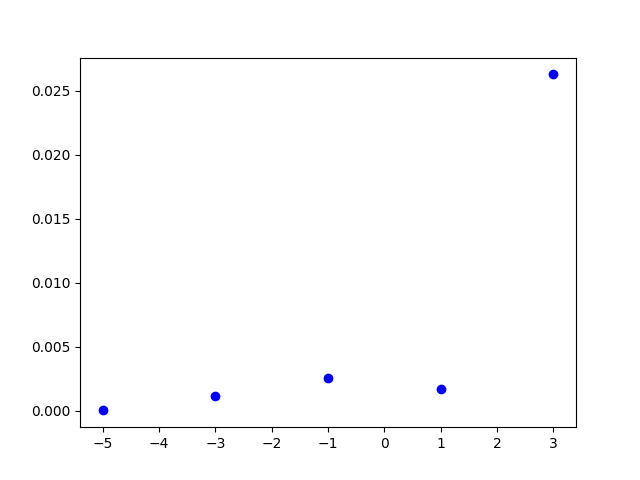
\includegraphics[scale=0.5]{p13.png}
\end{center}
$||\bm{w}||$ has the largest value when $\log_{10}C = 3$ and stays the same on the rest four $C$.

\section*{14}
\begin{center}
    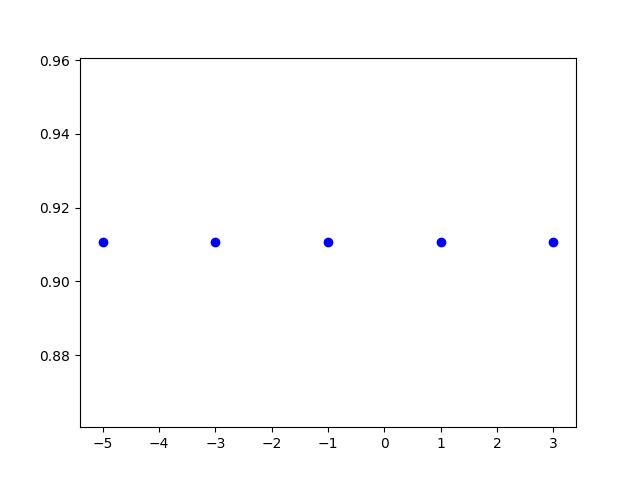
\includegraphics[scale=0.5]{p14.png}
\end{center}
$E_{in}$ remains the same for each $C$.
Which means that the SVM models with different $C$ have the same performance on training samples.

\section*{15}
\begin{center}
    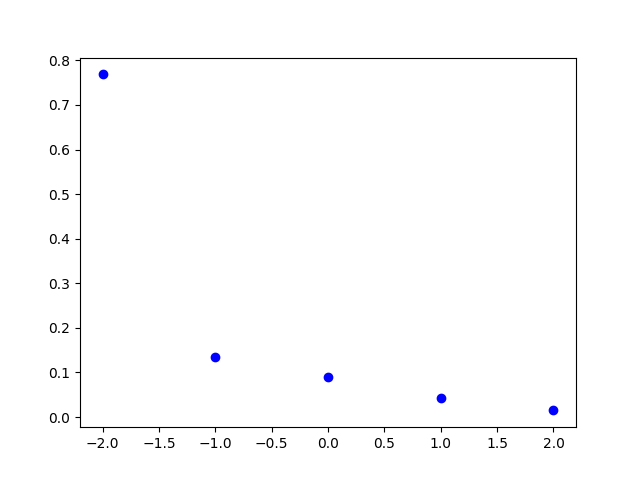
\includegraphics[scale=0.5]{p15.png}
\end{center}
The distance between free support vectors and hyperplane has the largest save when $C = 0.01$.
This verifies the intuition of soft-margin SVM objective function, 
smaller $C$ means smaller penalty and larger margin.

\section*{16}
\begin{center}
    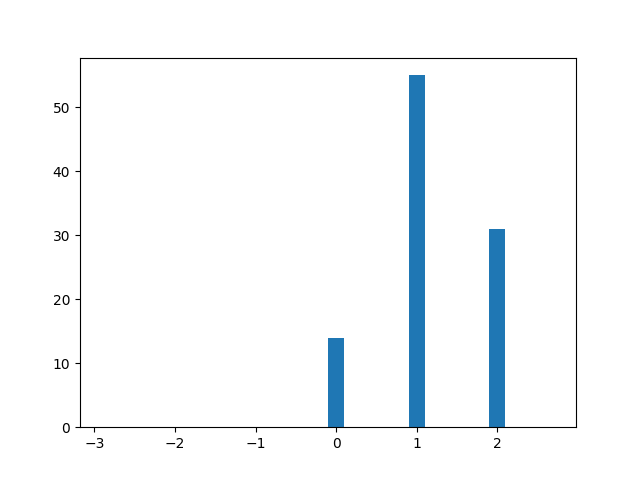
\includegraphics[scale=0.5]{p16.png}
\end{center}
Only the models with $\gamma = 1, 10, 100$ are selected. Through validation, $\gamma = 10$ seems to have best performance.

\section*{17}
In dual SVM KKT condition, we know that
\begin{equation}
    w_i = \sum_{i=1}^{N} \alpha_n y_n z_{n,i}
\end{equation}
and 
\begin{equation}
    \sum_{i=1}^{N} \alpha_n y_n = 0
\end{equation}

\begin{equation*}
\begin{split}
    w_0 &= \sum_{i=1}^{N} \alpha_n y_n z_{n,0} \\
    &=  z_{n,0} \sum_{i=1}^{N} \alpha_n y_n = 0
\end{split}
\end{equation*}


\section*{18}
Assume that the new objective function is 
\[  \frac{1}{2} \bm{\alpha}'^T Q' \bm{\alpha}' - \mathbbm{1}^T \bm{\alpha}' \]
which $Q' = Q + q \cdot \bm{y} \bm{y}^T$ because of 
\[ 
    Q'_{n,m} 
    = y_n y_m \tilde{K}(x_n, y_n)
    = y_n y_m K(x_n, y_n) + q y_n y_m
\]
We also know that $\sum_{i=1}^{N} \alpha'_i y_i = 0$ and so $\bm{y}^T\bm{\alpha}' = 0$.
\begin{equation*}
    \begin{split}
        \frac{1}{2} \bm{\alpha}'^T Q' \bm{\alpha}' - \mathbbm{1}^T \bm{\alpha}'
        &= \frac{1}{2} \bm{\alpha}'^T (Q + q\bm{y} \bm{y}^T) \bm{\alpha}' - \mathbbm{1}^T \bm{\alpha}' \\
        &= \frac{1}{2} \bm{\alpha}'^T Q \bm{\alpha}' + \frac{1}{2} (\bm{y}^T\bm{\alpha}')(\bm{y}^T\bm{\alpha}')  - \mathbbm{1}^T \bm{\alpha}' \\
        &=  \frac{1}{2} \bm{\alpha}'^T Q \bm{\alpha}' - \mathbbm{1}^T \bm{\alpha}'
    \end{split}
\end{equation*}
The new objective function is equivalent to the original one. Therefore, the support vectors for each SVM are the same and $\alpha_i' = \alpha_i$
The new decision function $f'(x)$ is the same as $f(x)$.

\begin{equation*}
    \begin{split}
        f'(x) &= \sum_{\text{SV indices n}} \alpha_n' y_n \tilde{K}(x_n, x) + y_s - \sum_{\text{SV indices n}} \alpha_n' y_n \tilde{K}(x_n, x_s) \\
        &= \bigg( \sum_{\text{SV indices n}} \alpha_n' y_n K(x_n, x) + q\sum_{\text{SV indices n}} \alpha_n'y_n \bigg) \\ 
        &+ y_s - \bigg( \sum_{\text{SV indices n}} \alpha_n' y_n K(x_n, x_s) + q\sum_{\text{SV indices n}} \alpha_n'y_n \bigg) \\
        &= \sum_{\text{SV indices n}} \alpha_n y_n K(x_n, x) + y_s - \sum_{\text{SV indices n}} \alpha_n y_n K(x_n, x_s) \\
        &= f(x)
    \end{split}
\end{equation*}
which $(x_s, y_s)$ is a free support vector.


\end{document}


